\documentclass[10pt,a4paper]{article}
\usepackage[utf8]{inputenc}
\usepackage[T1]{fontenc}
\usepackage{amsmath}
\usepackage[brazilian]{babel}
\usepackage[margin=1.6cm]{geometry}
\usepackage{multicol}
\usepackage{graphicx}
\usepackage{booktabs}
\usepackage{float}
\usepackage{xcolor}
\usepackage{mathptmx}
\usepackage{listings}

\definecolor{cmt}{rgb}{0.0,0.5,0.0}
\definecolor{kw}{rgb}{0.0,0.0,0.7}
\definecolor{str}{rgb}{0.6,0.1,0.1}
\definecolor{gry}{gray}{0.5}
\lstset{language=C, basicstyle=\ttfamily\scriptsize, keywordstyle=\color{kw},
  commentstyle=\color{cmt}\itshape, stringstyle=\color{str},
  numbers=left, numberstyle=\tiny\color{gry}, numbersep=6pt,
  breaklines=true, breakatwhitespace=false, showstringspaces=false,
  frame=single, framesep=4pt, tabsize=4, xleftmargin=14pt,
  morekeywords={omp,pragma}}

\setlength{\parindent}{0pt}
\setlength{\parskip}{3pt}
\pagestyle{plain}
\begin{document}

\begin{center}
  {\Large\bfseries Cálculo Paralelo do Conjunto de Mandelbrot com MPI + OpenMP}\\[3pt]
  {\large Versão híbrida: MPI Coordenador/Trabalhador entre nós e \emph{workpool} OpenMP (sem mestre) dentro do nó}\\[6pt]
  Bernardo Luiz Padilha Zamin \quad\textbullet\quad João Pedro Sostruznik Sotero da Cunha\\[2pt]
  {\small Programação Paralela --- Trabalho 4 (MPI + OpenMP), PUCRS --- Escola Politécnica, 2026}
\end{center}
\vspace{2pt}\hrule\vspace{8pt}

\begin{multicols}{2}

\section*{1. Introdução}
Implementa-se, em C, a versão \textbf{híbrida MPI + OpenMP} do cálculo do \textbf{conjunto de Mandelbrot} (imagem \textbf{7680$\times$4320}), reaproveitando o \emph{Coordenador/Trabalhador} do grupo. São \textbf{dois níveis de paralelismo}: o \textbf{MPI} distribui blocos de linhas entre os \textbf{nós} (\textbf{um processo pesado por nó}) e o \textbf{OpenMP} usa os núcleos \emph{dentro} de cada nó no modelo \textbf{workpool sem mestre}. Avaliam-se \emph{speed-up}, eficiência e escalabilidade \textbf{forte} e \textbf{fraca} em até \textbf{4 nós}, o efeito do \textbf{Hyper-Threading}, as \textbf{formas de alocar o coordenador} e a \textbf{comparação com a MPI pura}.

\section*{2. Modelo híbrido}
\textbf{Entre nós (MPI).} Modelo \textbf{Coordenador/Trabalhador} \emph{idêntico} ao da MPI pura, preservando a comparabilidade. O \texttt{rank 0} distribui \textbf{blocos de \texttt{rows\_per\_task} linhas sob demanda}: o trabalhador pede (\texttt{TAG\_REQUEST}), recebe \texttt{TAG\_TASK} (tarefa) ou \texttt{TAG\_STOP} (fim), calcula e devolve (\texttt{TAG\_RESULT}). Há \textbf{um processo pesado por nó}, com todos os núcleos do nó à disposição das threads. Para cada pixel itera-se $z\leftarrow z^2+c$ até $|z|>2$ ou \texttt{max\_iter}; pontos \emph{internos} custam \texttt{max\_iter} e \emph{externos} terminam cedo, gerando \textbf{carga irregular} que exige \textbf{balanceamento dinâmico}.

\section*{3. Workpool OpenMP sem mestre}
Cada bloco é processado por uma \textbf{região paralela} (\texttt{\#pragma omp parallel}). O controle está numa \textbf{estrutura de dados compartilhada} \texttt{WorkPool\{next,total\}}: \textbf{todas as threads} executam o mesmo laço e \textbf{retiram atomicamente} a próxima linha (\texttt{\#pragma omp atomic capture}) até esvaziar o pool --- \textbf{sem thread mestre}, com escalonamento \emph{self-service} emergindo da estrutura de dados (modelo \emph{workpool}/\emph{bag-of-tasks}). A granularidade é de \textbf{uma linha} (7680 px), que amortiza a sincronização e ainda equilibra a carga. Usa-se \texttt{MPI\_Init\_thread} (\texttt{MPI\_THREAD\_FUNNELED}; só a thread principal chama MPI) e \texttt{OMP\_NUM\_THREADS=16} (8 núcleos $\times$ 2 HT).

\section*{4. Alocação do coordenador}
O coordenador só distribui/coleta, ficando \textbf{quase ocioso}. Há duas alocações, escolhidas \textbf{sem alterar o código} (via SLURM, \texttt{-n 4} vs \texttt{-n 5}): \emph{dedicada} --- ocupa um nó inteiro (em 4 nós sobram 3 trabalhadores e o nó do coordenador fica ocioso); e \emph{compartilhada} --- divide o nó com um trabalhador (4 trabalhadores em 4 nós).

\section*{5. Metodologia}
Até \textbf{4 nós} da Atlantica (LAD), SLURM, Xeon E5520, \textbf{16 CPUs lógicas/nó} (8 núcleos $\times$ 2 HT). \texttt{ladcomp -env mpicc -O3 -fopenmp}. Tempo por \texttt{MPI\_Wtime} \emph{antes} do I/O. Baseline $T(1)=93{,}19$\,s (sequencial, \texttt{max\_iter}=2000). \textbf{Forte}: \texttt{max\_iter} fixo, variando recursos. \textbf{Fraca}: \texttt{max\_iter}=1500$\times$workers. Speed-up$\,=T(1)/T(p)$; Eficiência$\,=$Speed-up$/p$. Saída \textbf{byte-idêntica} à sequencial (\texttt{md5}).

\section*{6. Resultados e análise}
\textbf{Workpool (Tab.\,1, Fig.\,a).} Escala quase linear até os 8 núcleos físicos (7,34$\times$, 92\%) e chega a \textbf{12,70$\times$} com 16 threads --- ganho de $\sim$73\% via \textbf{Hyper-Threading}, com \emph{todas} as threads ocupadas apesar da carga irregular.

\textbf{Escalabilidade forte (Tab.\,3, Fig.\,b).} O híbrido atinge \textbf{31$\times$ em 4 nós}. A eficiência cai em 4 nós (0,65) porque o tempo já é de $\sim$3\,s e o \textbf{custo fixo} --- MPI e a \textbf{coleta da imagem de $\sim$127\,MB} no coordenador ($O(N)$, independe de $p$) --- domina (Amdahl); com carga maior aproxima-se do ideal.

\textbf{Alocação do coordenador (Fig.\,c, Tab.\,4).} Dedicar um nó ao coordenador ocioso \textbf{desperdiça 1/4 dos recursos}; \emph{compartilhar} (4 trabalhadores) reduz o tempo de \textbf{2,96 para 2,35\,s --- 20,7\% mais rápido}.

\textbf{Híbrido $\times$ MPI pura (Tab.\,4).} Nesta escala \emph{compute-bound}, a \textbf{MPI pura com HT} (64 proc., todos os 4 nós calculando) é a mais rápida (\textbf{2,00\,s, 46,5$\times$}); o híbrido \emph{compartilhado} fica competitivo (2,35\,s, 39,7$\times$) e o \emph{dedicado} perde por ociosar um nó. As vantagens do híbrido --- menos \emph{ranks}, menos memória e mensagens --- surgem em \textbf{escalas maiores} ou com mais comunicação.

\textbf{Escalabilidade fraca (Tab.\,2, Fig.\,d).} Com carga proporcional aos trabalhadores, o tempo permanece \textbf{praticamente constante} (5,1--5,4\,s), com eficiência \textbf{97--104\%} --- próximo do ideal.

\section*{7. Conclusão}
A versão cumpre o modelo: \textbf{MPI Coordenador/Trabalhador} (um processo por nó) + \textbf{workpool OpenMP sem mestre} (controle por estrutura de dados, uma thread por núcleo lógico, HT). O \emph{workpool} escala bem no nó (12,7$\times$) e a escalabilidade \textbf{fraca} é quase ideal. \textbf{Dedicar um nó ao coordenador é desvantajoso} (compartilhar é 20,7\% melhor). Em pequena escala \emph{compute-bound} a \textbf{MPI pura} vence em tempo bruto; o híbrido fica competitivo ao compartilhar o coordenador e tende a ganhar em escalas maiores.

\end{multicols}

\newpage
\begin{center}\textbf{Tabelas e gráfico}\end{center}

\begin{multicols}{2}
\begin{center}
\textbf{Tabela 1 --- Workpool OpenMP (1 nó)}\\[3pt]
\begin{tabular}{rrrr}
\toprule
Threads & Tempo (s) & Speed-up & Efic. \\ \midrule
1  & 87,01 & 1,00  & 1,00 \\
2  & 43,68 & 1,99  & 1,00 \\
4  & 23,40 & 3,72  & 0,93 \\
8  & 11,85 & 7,34  & 0,92 \\
16 &  6,85 & 12,70 & 0,79 \\ \bottomrule
\end{tabular}

\vfill\columnbreak
\textbf{Tabela 2 --- Escalabilidade fraca}\\[3pt]
\begin{tabular}{lrrr}
\toprule
Nós & \texttt{max\_iter} & Tempo (s) & Efic. \\ \midrule
2 (1 w.) & 1500 & 5,25 & 1,00 \\
3 (2 w.) & 3000 & 5,06 & 1,04 \\
4 (3 w.) & 4500 & 5,40 & 0,97 \\ \bottomrule
\end{tabular}
\end{center}
\end{multicols}

\begin{center}
\textbf{Tabela 3 --- Escalabilidade forte: híbrido $\times$ MPI pura (HT)}\\[3pt]
\begin{tabular}{r rrr rrr}
\toprule
 & \multicolumn{3}{c}{Híbrido (1 proc/nó, 16 threads)} & \multicolumn{3}{c}{MPI pura (16 proc/nó)} \\
\cmidrule(lr){2-4}\cmidrule(lr){5-7}
nós & Tempo (s) & Speed-up & Efic. & Tempo (s) & Speed-up & Efic. \\ \midrule
2 & 7,08 & 13,2 & 0,82 & 3,35 & 27,8 & 0,87 \\
3 & 3,45 & 27,0 & 0,84 & 2,74 & 34,1 & 0,71 \\
4 & 2,96 & 31,5 & 0,66 & 2,00 & 46,5 & 0,73 \\ \bottomrule
\end{tabular}
\end{center}

\vspace{3pt}
\begin{center}
\textbf{Tabela 4 --- Comparação em 4 nós (alocação do coordenador e híbrido $\times$ MPI)}\\[3pt]
\begin{tabular}{lrrr}
\toprule
Configuração & Processos & Tempo (s) & Speed-up \\ \midrule
MPI pura (HT, todos os nós calculando)       & 64           & \textbf{2,00} & \textbf{46,5} \\
Híbrido --- coordenador \emph{compartilhado} & 4 nós (4 w.) & 2,35          & 39,7 \\
Híbrido --- coordenador \emph{dedicado}      & 4 nós (3 w.) & 2,96          & 31,5 \\
MPI pura (1 processo por núcleo físico)      & 32           & 3,20          & 29,1 \\ \bottomrule
\end{tabular}
\end{center}

{\small $T(1)=93{,}19$\,s (sequencial, 1 núcleo, \texttt{max\_iter}=2000); Speed-up$\,=T(1)/T(p)$; Eficiência$\,=$Speed-up$/p$, $p=$ núcleos lógicos de cálculo (híbrido: trabalhadores$\times$16; MPI pura: nº de processos). Imagem 7680$\times$4320. Fraca: eficiência $=T(\text{1 trab.})/T(p)$.}

\vspace{5pt}
\begin{center}
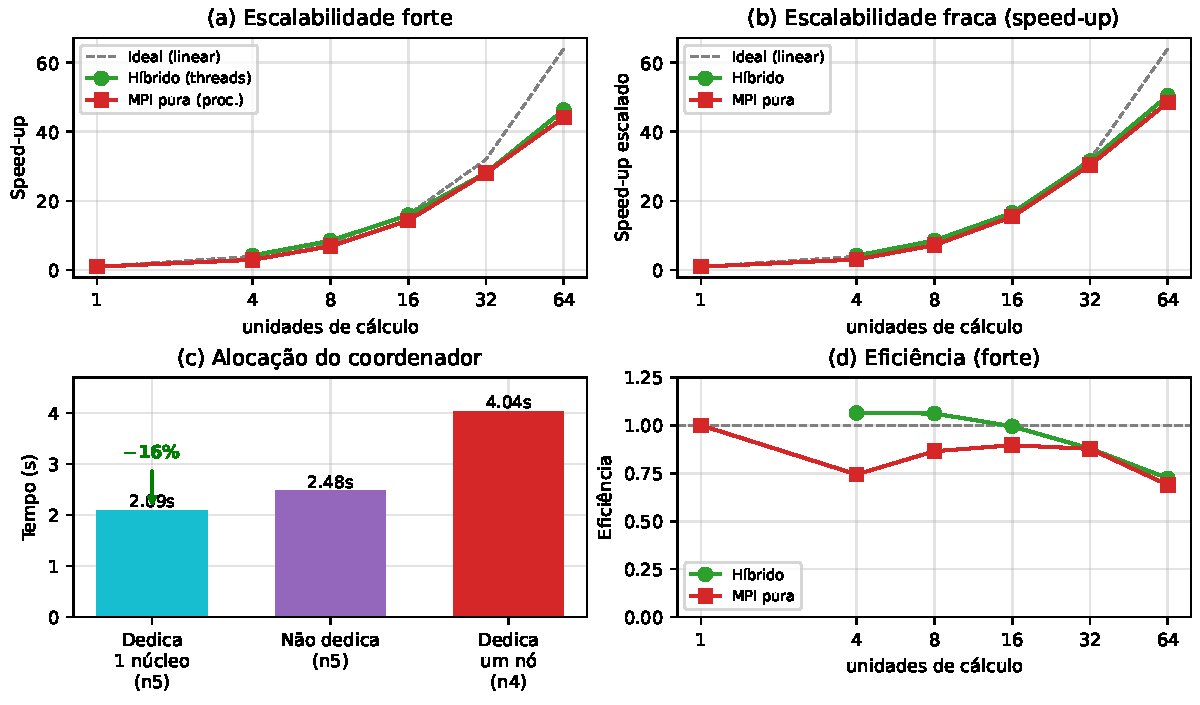
\includegraphics[width=0.86\linewidth]{graficos.pdf}\\[2pt]
{\small Figura 1 --- (a) \emph{workpool} OpenMP dentro de um nó (speed-up $\times$ threads); (b) escalabilidade forte, híbrido $\times$ MPI pura; (c) alocação do coordenador; (d) escalabilidade fraca.}
\end{center}

\newpage
\begin{center}{\large\bfseries Anexo --- Código-fonte (\texttt{mandelbrot-hib.c}, trechos relevantes)}\end{center}
\vspace{3pt}
\textbf{Versão híbrida MPI + OpenMP.} O coordenador (\texttt{rank 0}) distribui blocos de linhas sob demanda e coleta os resultados (idêntico ao \texttt{mandelbrot-mpi.c}); cada trabalhador calcula seu bloco com o \emph{workpool} OpenMP (\texttt{compute\_task\_workpool}, \emph{sem mestre}). As funções inalteradas (\texttt{mandelbrot}, \texttt{save\_ppm}) e o laço do coordenador são omitidos por brevidade. Compilação: \texttt{ladcomp -env mpicc -O3 mandelbrot-hib.c -o mandelbrot-hib -fopenmp -lm}.
\nopagebreak
\begin{lstlisting}
#include <mpi.h>
#include <omp.h>
#include <stdio.h>
#include <stdlib.h>
#include <math.h>
#define WIDTH  7680
#define HEIGHT 4320
#define DEFAULT_ROWS_PER_TASK 64
#define TAG_REQUEST 0
#define TAG_TASK    1
#define TAG_RESULT  2
#define TAG_STOP    3
typedef struct { int start_row; int num_rows; } Task;
/* Estrutura de dados compartilhada que CONTROLA o workpool (sem mestre):
   next = indice da proxima linha do bloco ainda nao tomada. */
typedef struct { int next; int total; } WorkPool;
int  mandelbrot(double real, double imag, int max_iter); /* z=z^2+c; igual ao seq/MPI */
void save_ppm(const char *f, int *img, int max_iter);    /* igual ao seq/MPI */
/* ===== WORKPOOL OpenMP: todas as threads trabalham, SEM MESTRE ===== */
void compute_task_workpool(const Task *task, int *buffer, int max_iter)
{
    WorkPool pool = { .next = 0, .total = task->num_rows };
    #pragma omp parallel                  /* todas as threads entram e trabalham */
    {
        while (1) {
            int row;
            #pragma omp atomic capture    /* retira atomicamente a proxima linha */
            { row = pool.next; pool.next++; }  /* do pool compartilhado (sem mestre) */
            if (row >= pool.total) break;      /* pool vazio: esta thread termina */
            int y = task->start_row + row;
            for (int x = 0; x < WIDTH; x++) {
                double real = -2.5 + (3.5 * x / WIDTH);
                double imag = -1.0 + (2.0 * y / HEIGHT);
                buffer[row * WIDTH + x] = mandelbrot(real, imag, max_iter);
            }
        }
    }
}
int main(int argc, char *argv[])
{
    int max_iter      = atoi(argv[1]);
    int rows_per_task = (argc >= 3) ? atoi(argv[2]) : DEFAULT_ROWS_PER_TASK;
    int provided;                         /* so a thread principal chama MPI */
    MPI_Init_thread(&argc, &argv, MPI_THREAD_FUNNELED, &provided);
    int rank, size;
    MPI_Comm_rank(MPI_COMM_WORLD, &rank);
    MPI_Comm_size(MPI_COMM_WORLD, &size);
    if (rank == 0) {
        /* COORDENADOR: distribui blocos sob demanda (TAG_TASK) e coleta os
           resultados (TAG_RESULT); cronometra (MPI_Wtime) e grava a imagem.
           Identico ao mandelbrot-mpi.c (laco MPI_Probe / MPI_Recv / MPI_Send). */
    } else {
        /* TRABALHADOR: pede tarefa, calcula com o workpool, devolve. */
        MPI_Status st; int request = 1;
        while (1) {
            MPI_Send(&request, 1, MPI_INT, 0, TAG_REQUEST, MPI_COMM_WORLD);
            Task task;
            MPI_Recv(&task, sizeof(Task), MPI_BYTE, 0, MPI_ANY_TAG,
                     MPI_COMM_WORLD, &st);
            if (st.MPI_TAG == TAG_STOP) break;
            int *buffer = malloc(sizeof(int) * task.num_rows * WIDTH);
            compute_task_workpool(&task, buffer, max_iter);   /* <== OpenMP */
            MPI_Send(&task,  sizeof(Task), MPI_BYTE, 0, TAG_RESULT, MPI_COMM_WORLD);
            MPI_Send(buffer, task.num_rows * WIDTH, MPI_INT, 0, TAG_RESULT,
                     MPI_COMM_WORLD);
            free(buffer);
        }
    }
    MPI_Finalize();
    return 0;
}
\end{lstlisting}

\end{document}
